% ============================================================
% Beamer — ISLP Lecture Series — IMPROVED EDITION
% Advanced Module A2: Explainable AI with Shapley Values
% ============================================================
\documentclass[aspectratio=169,11pt]{beamer}
\usepackage[utf8]{inputenc}\usepackage[T1]{fontenc}\usepackage[english]{babel}
\usepackage{graphicx}\usepackage{booktabs}\usepackage{amsmath,amssymb,amsfonts}
\usepackage{mathtools}\usepackage{hyperref}\usepackage{xcolor}
\usepackage{verbatim}\usepackage{alltt}
\usepackage{tikz}\usetikzlibrary{calc,arrows.meta,positioning,shapes}
\usepackage{tcolorbox}\tcbuselibrary{skins}

\usetheme{Madrid}\usecolortheme{default}
\setbeamertemplate{navigation symbols}{}
\setbeamertemplate{footline}[frame number]
\setbeamertemplate{blocks}[rounded][shadow=false]
\setbeamertemplate{headline}{%
  \leavevmode\hbox{%
    \begin{beamercolorbox}[wd=\paperwidth,ht=2.2ex,dp=0.9ex]{section in head/foot}%
      {\fontsize{4.6}{5.2}\selectfont%
       \insertsectionnavigationhorizontal{\paperwidth}{}{\hskip0pt plus1filll}}%
    \end{beamercolorbox}}%
}
\setbeamerfont{section in head/foot}{size=\tiny}
\setbeamerfont{palette primary}{size=\tiny}
\setbeamerfont{palette tertiary}{size=\tiny}
\setbeamerfont{section in toc}{size=\footnotesize}

\usepackage{listings}
\definecolor{pyKw}{RGB}{0,0,180}\definecolor{pyStr}{RGB}{20,120,40}
\definecolor{pyCom}{RGB}{120,120,120}\definecolor{accent}{RGB}{38,70,140}
\lstdefinestyle{Pystyle}{language=Python,basicstyle=\ttfamily\footnotesize,
  keywordstyle=\color{pyKw}\bfseries,commentstyle=\color{pyCom}\itshape,
  stringstyle=\color{pyStr},showstringspaces=false,upquote=true,
  columns=fullflexible,breaklines=true,literate={~}{{$\sim$}}1}
\lstset{style=Pystyle}

% Tighter TOC spacing (place AFTER \lstset, BEFORE \AtBeginSection)
\usepackage{etoolbox}
\makeatletter
\patchcmd{\beamer@sectionintoc}{\vskip1.5em}{\vskip.6em}{\typeout{TOCPATCH-OK}}{\typeout{TOCPATCH-FAIL}}
\makeatother

\AtBeginSection[]{\begin{frame}{Outline}\footnotesize
  \tableofcontents[currentsection,sectionstyle=show/shaded,subsectionstyle=show/show/hide]
\end{frame}}

\newcommand{\islpsource}[1]{%
  \vfill\hfill{\tiny\itshape\color{gray}Source: #1 \textemdash{} ISLP, James et al.\ (2023).}\par
}

\newtcolorbox{takeaway}[1][Takeaway]{enhanced,colback=green!4,colframe=green!50!black,
  boxrule=0pt,leftrule=2.5pt,arc=2pt,fonttitle=\bfseries,title=#1,
  left=2mm,right=2mm,top=1mm,bottom=1mm}
\newtcolorbox{numexample}[1][Worked example]{enhanced,colback=orange!4,colframe=orange!70!black,
  boxrule=0pt,leftrule=2.5pt,arc=2pt,fonttitle=\bfseries,title=#1,
  left=2mm,right=2mm,top=1mm,bottom=1mm}
\newtcolorbox{readme}[1][How to read this]{enhanced,colback=blue!4,colframe=accent,
  boxrule=0pt,leftrule=2.5pt,arc=2pt,fonttitle=\bfseries,title=#1,
  left=2mm,right=2mm,top=1mm,bottom=1mm}

\title{Quantitative Research Methods}
\subtitle{Explainable AI with Shapley Values\\[2pt]{\small Advanced module A2 --- optional self-study}}
\author{Prof.\ Dr.\ Christoph Weisser}
\date{}\graphicspath{{images/}}

\newtcolorbox{exercise}[1][Exercise]{enhanced, fontupper=\footnotesize, colback=purple!4, colframe=purple!55!black, boxrule=0pt, leftrule=2.5pt, arc=2pt, fonttitle=\bfseries, title=#1, left=2mm, right=2mm, top=1mm, bottom=1mm}
\newtcolorbox{solutionbox}[1][Solution]{enhanced, fontupper=\footnotesize, colback=teal!5, colframe=teal!55!black, boxrule=0pt, leftrule=2.5pt, arc=2pt, fonttitle=\bfseries, title=#1, left=2mm, right=2mm, top=1mm, bottom=1mm}
\newtcolorbox{longexercise}[1][Extended exercise (15 min)]{enhanced, fontupper=\footnotesize, colback=violet!6, colframe=violet!55!black, boxrule=0pt, leftrule=3pt, arc=2pt, fonttitle=\bfseries, title=#1, left=2mm, right=2mm, top=1mm, bottom=1mm}

% Reclaim ~2pt of body height (custom nav headline makes full slides tip over by ~1.83pt)
\addtobeamertemplate{frametitle}{}{\vspace{-2pt}}

\newtcolorbox{labnote}[1][Run this live in the lab notebook]{enhanced, fontupper=\footnotesize, colback=cyan!7, colframe=cyan!45!black, boxrule=0pt, leftrule=3pt, arc=2pt, fonttitle=\bfseries, title=#1, left=2mm, right=2mm, top=1mm, bottom=1mm}

% Common-mistake callout --- crimson, for the error to pre-empt
\newtcolorbox{mistake}[1][Common mistake]{enhanced, fontupper=\footnotesize, colback=red!4, colframe=red!60!black, boxrule=0pt, leftrule=3pt, arc=2pt, fonttitle=\bfseries, title=#1, left=2mm, right=2mm, top=1mm, bottom=1mm}

\begin{document}

\begin{frame}[plain]\titlepage\end{frame}

\begin{frame}{Where this module fits}
  \footnotesize
  This is one of four \textbf{optional advanced modules} that extend the core course.
  Nothing here is exam material for the main chapters --- but everything here is built
  from tools you already own.
  \begin{center}
  \begin{tabular}{@{}lll@{}}
    \toprule
    \textbf{You already know} & \textbf{From} & \textbf{Used here for} \\
    \midrule
    Flexibility vs.\ interpretability & Ch.\ 2 & why accurate models need explaining \\
    Boosting, variable importance & Ch.\ 8 & the black box we explain; the benchmark \\
    Deep networks & Ch.\ 10 & the archetypal black box (same machinery) \\
    The $2^p$ subset count & Ch.\ 0b, Ch.\ 6 & the cost of exact Shapley computation \\
    Seeded simulation, resampling & Ch.\ 5 & background samples, Monte-Carlo error \\
    \bottomrule
  \end{tabular}
  \end{center}
  \vspace{2pt}
  \begin{takeaway}[Today's question]
    Chapter 8 gave us a boosted model that predicts well; Chapter 10 gave us networks
    nobody can read. This module answers: \textbf{for one prediction, how much did each
    feature contribute --- exactly, with a guarantee?}
  \end{takeaway}
\end{frame}

\begin{frame}{Contents}\small\tableofcontents[hideallsubsections]
  \vfill
  {\tiny Optional and advanced material is collected in the \textbf{appendix} at the end of the deck.}
\end{frame}

\begin{frame}{Notation in this module}
  \footnotesize
  \begin{center}
  \begin{tabular}{@{}ll@{}}
    \toprule
    \textbf{Symbol} & \textbf{Meaning} \\
    \midrule
    $p$ & number of features (game-theory: players); here $p=6$ \\
    $\mathcal{P}=\{1,\dots,p\}$ & the grand coalition: all players together \\
    $S \subseteq \mathcal{P}\setminus\{j\}$ & a coalition (subset of players) not containing $j$; $|S|$ its size \\
    $v(S)$ & value function: the worth achieved by coalition $S$ alone \\
    $\varphi_j$ & Shapley value of player / feature $j$ \\
    $f(x)$ & the fitted model's prediction at input $x$ \\
    $x_S$ & the explained instance's values on the features in $S$ \\
    $X_{\bar S}$ & the random features \emph{outside} $S$ \\
    $\varphi_0$ & baseline: $E[f(X)]$, the average prediction \\
    $b^{(1)},\dots,b^{(B)}$ & background sample of $B$ rows (here $B=100$) \\
    $\pi$, $\mathrm{pre}_\pi(j)$ & a random ordering of the players; those placed before $j$ in $\pi$ \\
    $m$ & number of sampled orderings in Monte-Carlo estimation \\
    \bottomrule
  \end{tabular}
  \end{center}
\end{frame}

\begin{frame}{Sources and references}
  \footnotesize
  \begin{block}{Primary textbook (course background)}
    James, G., Witten, D., Hastie, T., Tibshirani, R., \& Taylor, J.\ (2023).
    \emph{An Introduction to Statistical Learning, with Applications in
    Python.} Springer. --- Chapters 8 and 10 supply the models we explain.
  \end{block}
  \begin{block}{Module sources}
    \begin{itemize}
      \item Shapley, L.\ S.\ (1953). A value for $n$-person games. \emph{Contributions to the Theory of Games II}, Princeton UP.
      \item \v{S}trumbelj, E., \& Kononenko, I.\ (2014). Explaining prediction models \dots{} with feature contributions. \emph{Knowledge and Information Systems}.
      \item Lundberg, S.\ M., \& Lee, S.-I.\ (2017). A unified approach to interpreting model predictions. \emph{NeurIPS} (the SHAP paper).
      \item Lundberg, S.\ M., et al.\ (2020). From local explanations to global understanding with explainable AI for trees. \emph{Nature Machine Intelligence} (TreeSHAP).
      \item Aas, K., Jullum, M., \& L{\o}land, A.\ (2021). Explaining individual predictions when features are dependent. \emph{Artificial Intelligence}.
      \item Molnar, C.\ (2022). \emph{Interpretable Machine Learning}, 2nd ed.\ (free online book).
    \end{itemize}
  \end{block}
\end{frame}

\begin{frame}{Learning objectives}
  By the end of this module you will be able to:
  \begin{itemize}
    \item \textbf{Distinguish} local from global explanations, and say what a
          feature attribution should promise.
    \item \textbf{Define} the Shapley value of a cooperative game and
          \textbf{verify} its four axioms on concrete numbers.
    \item \textbf{Translate} a fitted model into a game via the value function
          $v(S)$, and \textbf{defend} a choice between marginal and conditional
          expectations.
    \item \textbf{Implement} exact Shapley values from scratch ($2^p$
          enumeration) and their Monte-Carlo approximation, and \textbf{check}
          the efficiency axiom numerically.
    \item \textbf{Read} waterfall, global-importance and dependence displays,
          and \textbf{compare} them with Chapter 8's permutation importance.
    \item \textbf{Avoid} the three classic pitfalls: off-manifold evaluation,
          causal over-reading, and attribution instability.
  \end{itemize}
\end{frame}

\begin{frame}{Roadmap of this module}
  \begin{takeaway}[From a parlour game to a regulator-ready explanation]
    \begin{enumerate}
      \item Why accurate models need explaining; local vs.\ global.
      \item Cooperative games and the Shapley value: formula, axioms, a
            fully worked three-player game.
      \item From games to models: the value function $v(S)$ and the
            marginal-vs.-conditional choice.
      \item Computation: exact $2^p$ enumeration by hand, Monte-Carlo
            sampling, KernelSHAP and TreeSHAP.
      \item Reading the output: waterfall, mean $|\varphi_j|$, dependence
            plots --- against permutation importance.
      \item Pitfalls: correlated features, causation, instability ---
            and what industry regulation demands.
    \end{enumerate}
  \end{takeaway}
\end{frame}

\begin{frame}{Where this module is used in industry}
  \scriptsize
  \begin{center}
  \begin{tabular}{@{}p{2.6cm}p{5.2cm}p{4.6cm}@{}}
    \toprule
    \textbf{Sector} & \textbf{Concrete application} & \textbf{Which decision it drives} \\
    \midrule
    Consumer credit & Adverse-action reasons for each declined loan
      application & Which ``principal reasons'' are printed on the legally required notice \\
    Insurance & What drives an individual quote in a boosted tariff &
      Whether a rating factor stays in the filed tariff \\
    Healthcare & Which vitals and labs pushed a patient's deterioration
      score up & Whether the clinician escalates the alert or dismisses it \\
    \bottomrule
  \end{tabular}
  \end{center}
  \begin{takeaway}[All three must account for one prediction rather than the model as a whole]
    In each row an opaque ensemble beats the interpretable alternative, and a human
    downstream has to justify a \textbf{single} case --- one letter, one quote, one
    patient. Shapley values are the de-facto standard answer because they come with a
    guarantee no rival attribution has: the numbers \textbf{sum exactly} to
    $f(x)$ minus the baseline, so nothing in the decision is left unaccounted for.
  \end{takeaway}
\end{frame}

% ============================================================
\section{Why Explainability}
% ============================================================

\begin{frame}{Accurate models nobody can read}
  \footnotesize
  Chapters 8 and 10 ended with a trade: \textbf{accuracy up, readability gone}.
  \begin{numexample}[Our running model (built in this module)]
    A \texttt{GradientBoostingRegressor} predicting \textbf{log salary} on the
    \texttt{Hitters} data ($n=263$ players after dropping missing salaries,
    $p=6$ features) reaches \textbf{training $R^2 = 0.965$} --- using
    $100$ trees of depth $3$. That is roughly $800$ leaf rules added together:
    no coefficient table to read, no single split to point at.
  \end{numexample}
  \begin{readme}[What we can no longer answer (yet)]
    \begin{itemize}
      \item A player asks: \emph{why does the model pay me less than him?}
      \item A manager asks: \emph{which statistics drive salary overall?}
      \item An auditor asks: \emph{does the model use the feature you claim it ignores?}
    \end{itemize}
  \end{readme}
  \begin{takeaway}
    We refuse to trade the accuracy back. Instead we add an \textbf{explanation layer}
    on top of the fixed black box $f$ --- this module builds that layer with a guarantee.
  \end{takeaway}
\end{frame}

\begin{frame}{Local vs.\ global --- and what an attribution must promise}
  \footnotesize
  \begin{columns}[T]
    \column{0.48\textwidth}
    \begin{block}{Local explanation}
      For \textbf{one} instance $x$: how much did each feature value push
      \emph{this} prediction $f(x)$ away from the average prediction?
      \emph{(the declined applicant, the flagged transaction)}
    \end{block}
    \column{0.48\textwidth}
    \begin{block}{Global explanation}
      For the \textbf{whole} model: which features matter most \emph{on
      average} across all instances? \emph{(model validation, driver analysis)}
    \end{block}
  \end{columns}
  \vspace{2pt}
  \begin{readme}[What a feature attribution should mean]
    Numbers $\varphi_1,\dots,\varphi_p$, one per feature, such that:
    (i) they \textbf{sum exactly} to $f(x)-E[f(X)]$ --- no leftover, no double count;
    (ii) a feature the model \textbf{ignores} gets $0$;
    (iii) two features used \textbf{identically} get the same number.
    These wishes will become the Shapley \emph{axioms} --- and they pin down a
    \emph{unique} answer.
  \end{readme}
  \begin{takeaway}
    Shapley values are \textbf{local} objects; averaging $|\varphi_j|$ over many
    instances then buys the global picture. One machinery, both questions.
  \end{takeaway}
\end{frame}

\begin{frame}{Exercise A2.1 --- Local or global? [Concept]}
\begin{exercise}
  For each question, say whether it needs a \textbf{local} or a \textbf{global}
  explanation, and what the attribution numbers should sum to (if anything):
  \begin{enumerate}
    \item ``Why was \emph{my} loan declined?''
    \item ``Which features should we monitor for drift in production?''
    \item ``The model predicts salary $\$743$k for this veteran while the average
          prediction is $\$349$k --- what accounts for the gap?''
    \item ``Can we drop \texttt{PutOuts} from the pipeline without losing accuracy?''
  \end{enumerate}
\end{exercise}
\end{frame}

\begin{frame}{Solution --- Exercise A2.1}
\begin{solutionbox}
  \textbf{Method.} Ask \emph{whose} prediction is being discussed: one instance
  $\Rightarrow$ local; the model as a whole $\Rightarrow$ global.
  \begin{enumerate}
    \item \textbf{Local.} One applicant, one prediction. The attributions should sum to
          $f(x)-E[f(X)]$: the gap between \emph{this} score and the average score.
    \item \textbf{Global.} A property of the model over its input distribution;
          mean $|\varphi_j|$ across instances is a natural monitor. No sum constraint
          --- it is an average of magnitudes.
    \item \textbf{Local}, and the sum is pinned down exactly: on the log scale the
          $\varphi_j$ must add up to $\log 743 - \log 349 \approx 0.756$. (This is our
          running example --- we will compute those six numbers exactly.)
    \item \textbf{Global} --- but note the trap: a small mean $|\varphi_j|$ says the
          model \emph{currently} leans little on \texttt{PutOuts}, not that the feature
          is useless; after refitting without it, other correlated features may absorb
          its role.
  \end{enumerate}
\end{solutionbox}
\begin{mistake}
  Answering a local question with a global tool: telling the declined applicant
  ``income is the most important feature of our model'' explains the \emph{model},
  not \emph{their} decision.
\end{mistake}
\end{frame}

% ============================================================
\section{The Shapley Value}
% ============================================================

\begin{frame}{Cooperative games: players, coalitions, value}
  \scriptsize
  A \textbf{cooperative game} is a pair $(\mathcal{P}, v)$:
  \begin{block}{Definition}
    \begin{itemize}
      \item $\mathcal{P}=\{1,\dots,p\}$: a set of $p$ \textbf{players};
      \item $v : 2^{\mathcal{P}} \to \mathbb{R}$ with $v(\varnothing)=0$: a
            \textbf{value function} giving the worth $v(S)$ that any
            \textbf{coalition} $S\subseteq\mathcal{P}$ can achieve on its own.
    \end{itemize}
    The question: how should the grand coalition's worth $v(\mathcal{P})$ be
    \textbf{divided fairly} among the players?
  \end{block}
  \begin{readme}
    ``Fair'' must reflect \emph{contribution}: a player who adds a lot to every
    coalition they join deserves more. The natural raw material is the
    \textbf{marginal contribution} $v(S\cup\{j\})-v(S)$ --- what $j$ adds when
    joining the coalition $S$. The difficulty: this number \emph{depends on} $S$.
    Shapley's 1953 answer long predates machine learning --- airports still split runway
    costs across aircraft types with it --- and it is the formula we are about to build.
  \end{readme}
\end{frame}

\begin{frame}{A three-player game with concrete numbers}
  \footnotesize
  Three specialists found a consultancy: \textbf{A} (modeller), \textbf{B}
  (engineer), \textbf{C} (designer). Quarterly revenue (in $1\,000$\,\texteuro)
  for every possible team:
  \begin{numexample}[The full value function]
    \begin{center}
    \begin{tabular}{@{}lcccccccc@{}}
      \toprule
      $S$ & $\varnothing$ & $\{A\}$ & $\{B\}$ & $\{C\}$ & $\{A,B\}$ & $\{A,C\}$ & $\{B,C\}$ & $\{A,B,C\}$ \\
      \midrule
      $v(S)$ & $0$ & $120$ & $60$ & $0$ & $270$ & $150$ & $90$ & $300$ \\
      \bottomrule
    \end{tabular}
    \end{center}
    C earns \emph{nothing} alone, yet every team gains $30$ when C joins it
    ($150-120$, $90-60$, $300-270$): C's design work only pays off on top of a
    product. A and B together show \emph{synergy}: $270 > 120+60$.
  \end{numexample}
  \begin{takeaway}
    Naive splits fail: equal thirds ($100$ each) ignores that A alone is worth
    $120$; paying stand-alone values ($120,60,0$) only distributes $180$ of the
    $300$ and gives C nothing despite C's reliable $+30$. We need a rule that
    \textbf{averages marginal contributions over all ways a team can form}.
  \end{takeaway}
\end{frame}

\begin{frame}{The coalition lattice (native diagram)}
  \footnotesize
  \begin{center}
  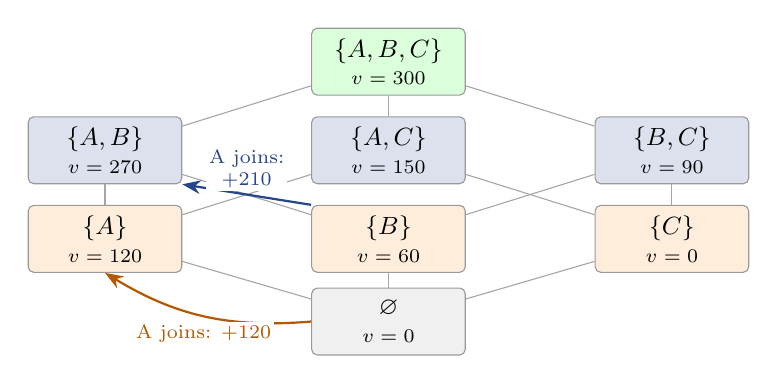
\begin{tikzpicture}[x=1cm,y=0.75cm,font=\small,
      co/.style={draw=black!40,rounded corners=2pt,minimum width=1.95cm,minimum height=0.85cm,align=center},
      ln/.style={black!35,thin}]
    \node[co,fill=green!14]  (ABC) at (0,4.4)  {$\{A,B,C\}$\\[-1pt]\scriptsize $v=300$};
    \node[co,fill=accent!16] (AB)  at (-3.6,2.9) {$\{A,B\}$\\[-1pt]\scriptsize $v=270$};
    \node[co,fill=accent!16] (AC)  at (0,2.9)  {$\{A,C\}$\\[-1pt]\scriptsize $v=150$};
    \node[co,fill=accent!16] (BC)  at (3.6,2.9)  {$\{B,C\}$\\[-1pt]\scriptsize $v=90$};
    \node[co,fill=orange!14] (A)   at (-3.6,1.4) {$\{A\}$\\[-1pt]\scriptsize $v=120$};
    \node[co,fill=orange!14] (B)   at (0,1.4)  {$\{B\}$\\[-1pt]\scriptsize $v=60$};
    \node[co,fill=orange!14] (C)   at (3.6,1.4)  {$\{C\}$\\[-1pt]\scriptsize $v=0$};
    \node[co,fill=black!6]   (E)   at (0,0)    {$\varnothing$\\[-1pt]\scriptsize $v=0$};
    \draw[ln] (E)--(A); \draw[ln] (E)--(B); \draw[ln] (E)--(C);
    \draw[ln] (A)--(AB); \draw[ln] (A)--(AC);
    \draw[ln] (B)--(AB); \draw[ln] (B)--(BC);
    \draw[ln] (C)--(AC); \draw[ln] (C)--(BC);
    \draw[ln] (AB)--(ABC); \draw[ln] (AC)--(ABC); \draw[ln] (BC)--(ABC);
    \draw[-{Stealth},accent,thick] (B.north west) -- (AB.south east)
      node[midway,above=1pt,fill=white,inner sep=1pt,align=center,
           font=\scriptsize\color{accent}] {A joins:\\$+210$};
    \draw[-{Stealth},orange!70!black,thick] (E.west) to[bend left=18]
      node[midway,below=2pt,fill=white,inner sep=1pt,
           font=\scriptsize] {A joins: $+120$} (A.south);
  \end{tikzpicture}
  \end{center}
  \begin{takeaway}
    Every edge is a marginal contribution. Player A adds $+120$ when joining the
    empty room but $+210$ when joining B ($270-60$): contributions
    \textbf{depend on who is already there}. The Shapley value will average over
    \emph{all} such edges, correctly weighted.
  \end{takeaway}
\end{frame}

\begin{frame}{Exercise A2.2 --- Fair division in the consultancy game [Math]}
\begin{exercise}
  Use the consultancy game
  ($v = 0, 120, 60, 0, 270, 150, 90, 300$ in the table order above).
  A player's Shapley value averages their marginal contribution over the six
  possible \textbf{arrival orders} $ABC, ACB, BAC, BCA, CAB, CBA$ (each equally
  likely).
  \begin{enumerate}
    \item Compute player A's marginal contribution in each of the six orders,
          and average them to get $\varphi_A$.
    \item Repeat for B and C (or use any shortcut you can justify).
    \item Verify \textbf{efficiency}: $\varphi_A+\varphi_B+\varphi_C = v(\{A,B,C\})$.
    \item Is C a \emph{dummy} player? Justify with one coalition.
  \end{enumerate}
\end{exercise}
\end{frame}

\begin{frame}{Solution --- Exercise A2.2 (1/2)}
\begin{solutionbox}[Solution --- the six arrival orders]
  \textbf{Method.} In an arrival order, each player's contribution is the jump in
  $v$ when they walk in. Tabulate all six orders once; then \emph{every} player's
  Shapley value is a column average of the same table.
  \begin{center}
  \begin{tabular}{@{}lccc@{}}
    \toprule
    Order & A adds & B adds & C adds \\
    \midrule
    $A\,B\,C$ & $120$ & $270-120=150$ & $300-270=30$ \\
    $A\,C\,B$ & $120$ & $300-150=150$ & $150-120=30$ \\
    $B\,A\,C$ & $270-60=210$ & $60$ & $300-270=30$ \\
    $B\,C\,A$ & $300-90=210$ & $60$ & $90-60=30$ \\
    $C\,A\,B$ & $150-0=150$ & $300-150=150$ & $0$ \\
    $C\,B\,A$ & $300-90=210$ & $90-0=90$ & $0$ \\
    \midrule
    mean & $\varphi_A=\tfrac{1020}{6}=\mathbf{170}$ & $\varphi_B=\tfrac{660}{6}=\mathbf{110}$ & $\varphi_C=\tfrac{120}{6}=\mathbf{20}$ \\
    \bottomrule
  \end{tabular}
  \end{center}
\end{solutionbox}
\end{frame}

\begin{frame}{Solution --- Exercise A2.2 (2/2)}
\begin{solutionbox}[Solution --- efficiency and the dummy check]
  \textbf{Part 3 --- efficiency.}
  \[
    \varphi_A+\varphi_B+\varphi_C = 170+110+20 = 300 = v(\{A,B,C\}). \checkmark
  \]
  The whole revenue is distributed --- nothing left over, nothing invented.

  \medskip
  \textbf{Part 4 --- is C a dummy?} \textbf{No.} A dummy adds nothing to \emph{any}
  coalition. But $v(\{A,C\})-v(\{A\}) = 150-120 = 30 \neq 0$: C adds $30$ to every
  non-empty team. C's stand-alone value is $0$, yet C's Shapley pay is $20>0$ ---
  the value correctly rewards \emph{team} contribution, not solo performance.

  \medskip
  \textbf{Comparison.} Equal thirds would overpay C ($100$ vs.\ $20$); stand-alone
  pay would underpay C ($0$) and fail efficiency ($180\ne300$). The order-averaged
  split is the only one we will be able to \emph{axiomatise}.
\end{solutionbox}
\begin{mistake}
  Computing marginal contributions only for the order $A,B,C$ and calling it a day.
  A single order is arbitrary --- A would get $120$ instead of $170$ --- and the
  result would depend on the labelling of the players.
\end{mistake}
\end{frame}

\begin{frame}{The Shapley value: the formula}
  \footnotesize
  \begin{block}{Rule (Shapley, 1953)}
    The Shapley value of player $j$ in the game $(\mathcal{P},v)$ is
    \[
      \boxed{\;\varphi_j \;=\; \sum_{S \,\subseteq\, \mathcal{P}\setminus\{j\}}
      \frac{|S|!\,\bigl(p-|S|-1\bigr)!}{p!}\;
      \Bigl(v\bigl(S\cup\{j\}\bigr)-v(S)\Bigr)\;}
    \]
  \end{block}
  \begin{readme}[Symbol by symbol]
    \begin{itemize}
      \item $S \subseteq \mathcal{P}\setminus\{j\}$ --- every coalition $j$ could join
            (all $2^{p-1}$ subsets not containing $j$);\quad
            $v(S\cup\{j\})-v(S)$ --- $j$'s \textbf{marginal contribution} on arrival.
      \item $|S|!$ --- arrival orders of $S$ \emph{before} $j$;\ $(p-|S|-1)!$ ---
            orders of the rest \emph{after} $j$;\ $p!$ --- all orders. So the weight is
            exactly $\Pr(\text{$j$ arrives right after the set } S)$ under a uniformly
            random order: the formula \emph{is} Exercise A2.2's order-averaging,
            written without listing orders.
      \item Equivalent form: weight $=\frac{1}{p}\binom{p-1}{|S|}^{-1}$ --- pick $j$'s
            arrival position first (each size equally likely), then the predecessors
            uniformly among that size.
    \end{itemize}
  \end{readme}
\end{frame}

\begin{frame}{Checking the formula on the consultancy game}
  \scriptsize
  \begin{numexample}[$\varphi_A {=} 170$ --- now via the subset formula ($p{=}3$)]
    Weights: $|S|=0:\ \tfrac{0!\,2!}{3!}=\tfrac13$;\quad
    $|S|=1:\ \tfrac{1!\,1!}{3!}=\tfrac16$;\quad
    $|S|=2:\ \tfrac{2!\,0!}{3!}=\tfrac13$.
    \begin{center}
    \begin{tabular}{@{}lcccc@{}}
      \toprule
      $S$ & weight & $v(S\cup\{A\})$ & $v(S)$ & term \\
      \midrule
      $\varnothing$ & $1/3$ & $120$ & $0$   & $40$ \\
      $\{B\}$       & $1/6$ & $270$ & $60$  & $35$ \\
      $\{C\}$       & $1/6$ & $150$ & $0$   & $25$ \\
      $\{B,C\}$     & $1/3$ & $300$ & $90$  & $70$ \\
      \midrule
      & & & $\varphi_A$ & $\mathbf{170}$ \\
      \bottomrule
    \end{tabular}
    \end{center}
    Same $170$ as the six-order average --- with $4$ terms instead of $6$ orders.
  \end{numexample}
  \begin{takeaway}
    Endpoint coalitions carry the \textbf{largest} weight ($\tfrac13$ each): one way to
    be first or last, $\binom{p-1}{|S|}$ ways to see a middle-sized crowd. For $p=6$:
    $\tfrac16, \tfrac1{30}, \tfrac1{60}, \tfrac1{60}, \tfrac1{30}, \tfrac16$ by size ---
    and for each $j$ the weights \textbf{sum to 1}: $\varphi_j$ is a weighted
    \emph{average} of marginal contributions.
  \end{takeaway}
\end{frame}


\begin{frame}{The Shapley value is an average, drawn}
  \begin{center}
    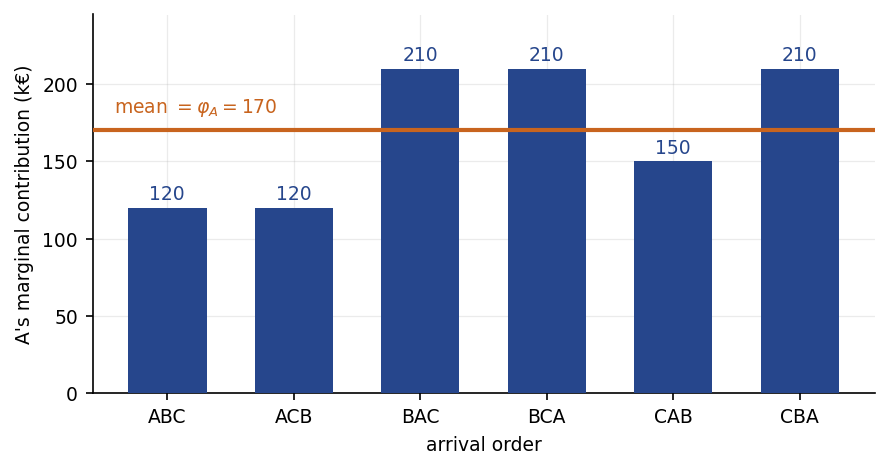
\includegraphics[width=0.72\textwidth,height=0.54\textheight,keepaspectratio]{a2_orders.png}
  \end{center}
  \begin{takeaway}
    A's marginal contribution in each of the $3! = 6$ arrival orders of the
    consultancy game. The Shapley value is nothing more mysterious than the
    \emph{mean of these bars} --- which is also why sampling orders
    (Monte-Carlo, later this module) estimates it unbiasedly.
  \end{takeaway}
\end{frame}

\begin{frame}{The four axioms --- and the uniqueness theorem}
  \footnotesize
  \begin{block}{Each axiom in one honest sentence}
    \begin{enumerate}
      \item \textbf{Efficiency:} the shares add up exactly,
            $\sum_{j=1}^{p}\varphi_j = v(\mathcal{P})-v(\varnothing)$ ---
            the whole surplus is distributed.
      \item \textbf{Symmetry:} if $v(S\cup\{i\})=v(S\cup\{j\})$ for every $S$
            containing neither, then $\varphi_i=\varphi_j$ --- equal treatment of
            interchangeable players.
      \item \textbf{Dummy (null player):} if $v(S\cup\{j\})=v(S)$ for every $S$,
            then $\varphi_j=0$ --- who never adds anything gets nothing.
      \item \textbf{Additivity:} for two games on the same players,
            $\varphi_j(v+w)=\varphi_j(v)+\varphi_j(w)$ --- playing two games at
            once changes nothing about either.
    \end{enumerate}
  \end{block}
  \begin{takeaway}[Why this matters]
    \textbf{Theorem (Shapley, 1953).} The Shapley value is the \emph{unique}
    allocation satisfying all four axioms. So once we accept the four wishes from
    the motivation slide, there is \textbf{no freedom left} --- the formula is not one
    heuristic among many, it is the only answer.
  \end{takeaway}
\end{frame}

\begin{frame}{Exercise A2.3 --- Weights and the dummy axiom [Math]}
\begin{exercise}
  Work directly with the weight $w(S) = \dfrac{|S|!\,(p-|S|-1)!}{p!}$.
  \begin{enumerate}
    \item For $p=3$, list $w(S)$ for all four coalitions
          $S\subseteq\{1,2,3\}\setminus\{j\}$ and show they sum to $1$.
    \item Prove the \textbf{dummy axiom} from the formula: if
          $v(S\cup\{j\})=v(S)$ for all $S$, then $\varphi_j=0$.
    \item Using $w(S)=\frac1p\binom{p-1}{|S|}^{-1}$, explain in one sentence why
          the empty and the almost-full coalition carry the largest weight.
  \end{enumerate}
\end{exercise}
\end{frame}

\begin{frame}{Solution --- Exercise A2.3}
\begin{solutionbox}
  \textbf{Part 1 --- the four weights for $p=3$.} The subsets of the other two
  players are $\varnothing$, two singletons, and the pair:
  \[
    w = \tfrac{0!\,2!}{3!},\ \tfrac{1!\,1!}{3!},\ \tfrac{1!\,1!}{3!},\ \tfrac{2!\,0!}{3!}
      = \tfrac13 + \tfrac16 + \tfrac16 + \tfrac13 = 1. \checkmark
  \]
  \textbf{Part 2 --- dummy.} Every term of
  $\varphi_j=\sum_S w(S)\,\bigl(v(S\cup\{j\})-v(S)\bigr)$ contains the factor
  $v(S\cup\{j\})-v(S)$, which is $0$ for every $S$ by assumption; a sum of zeros
  is $0$. (Because the weights sum to $1$, the same argument shows more: $\varphi_j$
  always lies between $j$'s smallest and largest marginal contribution.)

  \medskip
  \textbf{Part 3 --- endpoint weights.} Writing $w(S)=\frac1p\binom{p-1}{|S|}^{-1}$:
  each \emph{size} $|S|$ is equally likely ($1/p$), and that probability is shared
  equally among the $\binom{p-1}{|S|}$ coalitions of that size --- sizes $0$ and
  $p-1$ have only \emph{one} coalition each, so each keeps the full $1/p$.
\end{solutionbox}
\begin{mistake}
  Reading the weight as ``all $2^{p-1}$ coalitions are equally important''. They are
  not: for $p=6$ a single middle coalition carries weight $\tfrac1{60}$, the empty one
  $\tfrac16$ --- ten times more.
\end{mistake}
\end{frame}

% ============================================================
\section{Games to Models}
% ============================================================

\begin{frame}{Features are players: the value function of a prediction}
  \scriptsize
  Fix the trained model $f$ and one instance $x$ to explain. Let the
  \textbf{features be the players}; a coalition $S$ means ``these feature values
  are \emph{known} to be $x_S$''.
  \begin{block}{Rule (SHAP value function, marginal form)}
    \[
      \boxed{\;v_x(S) \;=\; E\bigl[f(x_S,\,X_{\bar S})\bigr] \;-\; E\bigl[f(X)\bigr]
      \;\approx\; \frac1B\sum_{b=1}^{B} f\bigl(x_S,\,x^{(b)}_{\bar S}\bigr) - \varphi_0\;}
    \]
    where $\varphi_0 = E[f(X)]$ and the expectation is estimated on a
    \textbf{background sample} $x^{(1)},\dots,x^{(B)}$.
  \end{block}
  \begin{readme}
    \begin{itemize}
      \item $f(x_S, X_{\bar S})$: evaluate the model with the \textbf{known}
            features pinned at $x$'s values and the \textbf{unknown} ones drawn
            from data --- an average prediction given what we know.
      \item $v_x(\varnothing)=0$ and $v_x(\mathcal{P})=f(x)-\varphi_0$: knowing
            nothing gives the average prediction; knowing everything gives $f(x)$.
      \item \textbf{Efficiency} then reads $\sum_j \varphi_j = f(x) - \varphi_0$:
            the attributions decompose \emph{this} prediction's distance from the
            average --- Lundberg \& Lee (2017) call this \emph{local accuracy},
            and SHAP $=$ \emph{SHapley Additive exPlanations}.
    \end{itemize}
  \end{readme}
\end{frame}

\begin{frame}{Marginal or conditional? The one modelling choice that matters}
  \scriptsize
  Two ways to ``not know'' the features outside $S$:
  \begin{columns}[T]
    \column{0.49\textwidth}
    \begin{block}{Marginal (interventional)}
      \[ v_x(S) = E\bigl[f(x_S, X_{\bar S})\bigr] - \varphi_0 \]
      Draw $X_{\bar S}$ from its own distribution, \textbf{ignoring} its
      correlation with $x_S$ --- like an intervention on the model's inputs.
    \end{block}
    \column{0.49\textwidth}
    \begin{block}{Conditional (observational)}
      \[ v_x(S) = E\bigl[f(X) \mid X_S = x_S\bigr] - \varphi_0 \]
      Draw $X_{\bar S}$ from its distribution \textbf{given} $X_S=x_S$ ---
      what we would expect from the data.
    \end{block}
  \end{columns}
  \vspace{2pt}
  \begin{readme}[Each option's honest price]
    \textbf{Marginal} respects the \emph{model}: unused features are true dummies
    ($\varphi_j=0$), but the average runs over feature combinations the data never
    produces (off-manifold --- pitfalls section). \textbf{Conditional} respects the
    \emph{data}: no impossible points, but correlated proxies of a used feature get
    credit even if the model never touches them --- the dummy axiom fails \emph{by
    design}, and the conditional distributions must themselves be estimated.
  \end{readme}
  \begin{takeaway}
    This module (like most software defaults) uses the \textbf{marginal} form: exact
    dummies, easy estimation --- and we will look its off-manifold problem in the eye.
  \end{takeaway}
\end{frame}

\begin{frame}{Our testbed: gradient boosting on \texttt{Hitters}}
  \footnotesize
  \begin{columns}[T]
    \column{0.56\textwidth}
    \begin{itemize}
      \item \textbf{Data:} \texttt{Hitters} --- $322$ baseball players (1986/87
            season); $59$ missing salaries dropped $\Rightarrow n=263$.
      \item \textbf{Target:} $\log(\texttt{Salary})$ (salaries in $\$1\,000$,
            range $67.5$--$2\,460$; the log tames the right tail).
      \item \textbf{Features ($p=6$):} \texttt{Years}, \texttt{CHits},
            \texttt{CRBI}, \texttt{Walks}, \texttt{Hits}, \texttt{PutOuts} ---
            small enough for \emph{exact} $2^6=64$-coalition Shapley.
      \item \textbf{Model:} \texttt{GradientBoostingRegressor} (sklearn defaults,
            \texttt{random\_state=2024}): training $R^2 = 0.965$.
      \item \textbf{Background:} $B=100$ rows drawn with
            \texttt{default\_rng(2024)}; baseline
            $\varphi_0 = 5.854$ log-dollars $\approx \$349$k.
    \end{itemize}
    \column{0.40\textwidth}
    \begin{numexample}[The instance we will explain]
      Row $188$: a \textbf{24-season veteran} holding the career-hits record ---
      \texttt{Years} $=24$, \texttt{CHits} $=4\,256$, \texttt{CRBI} $=1\,314$,
      \texttt{Walks} $=30$, \texttt{Hits} $=52$, \texttt{PutOuts} $=523$.
      Actual 1987 salary: $\$750$k. Model: $f(x)=6.610 \approx \$743$k.
    \end{numexample}
  \end{columns}
  \vspace{2pt}
  \begin{labnote}
    Section \S1--\S2 of \texttt{advanced\_02\_shapley\_lab.ipynb} loads
    \texttt{Hitters}, fits this exact model and builds the background sample ---
    run it now so the later cells have $f$, \texttt{bg} and \texttt{base} in memory.
  \end{labnote}
\end{frame}

\begin{frame}{Exercise A2.4 --- The duplicated feature [Concept]}
\begin{exercise}
  A bank's dataset accidentally contains \texttt{income} twice
  (\texttt{income\_a} $=$ \texttt{income\_b} for every customer). The fitted
  model happens to split \textbf{only} on \texttt{income\_a}.
  \begin{enumerate}
    \item Under the \textbf{marginal} value function, what is
          $\varphi_{\texttt{income\_b}}$? Which axiom decides it?
    \item Under the \textbf{conditional} value function, why does
          \texttt{income\_b} receive a non-zero share?
    \item Which of the two constructions evaluates the model at customer
          profiles that cannot exist (\texttt{income\_a} $\neq$
          \texttt{income\_b})?
    \item Give one question for which the marginal answer is the right one, and
          one for which the conditional answer is.
  \end{enumerate}
\end{exercise}
\end{frame}

\begin{frame}{Solution --- Exercise A2.4}
\begin{solutionbox}
  \textbf{Part 1.} $\varphi_{\texttt{income\_b}} = 0$ by the \textbf{dummy axiom}:
  the model never touches \texttt{income\_b}, so pinning it changes no prediction,
  so every marginal contribution is $0$.

  \smallskip
  \textbf{Part 2.} Conditioning on $\texttt{income\_b}=x$ forces
  $\texttt{income\_a}=x$ too (they are identical), so
  $E[f(X)\mid \texttt{income\_b}]$ moves exactly as much as conditioning on
  \texttt{income\_a} --- informationally the twins are symmetric, and they share
  the credit. The dummy axiom fails, \emph{deliberately}.

  \smallskip
  \textbf{Part 3.} The \textbf{marginal} one: computing
  $v(\{\texttt{income\_a}\})$ it pins \texttt{income\_a} at the customer's value
  while drawing \texttt{income\_b} from the background --- creating profiles with
  two different incomes, which the data manifold does not contain.

  \smallskip
  \textbf{Part 4.} \emph{``Does the deployed model discriminate on
  \texttt{income\_b}?''} --- marginal (mechanistic: no, it cannot).
  \emph{``Does the score reveal / depend on the information in
  \texttt{income\_b}?''} --- conditional (informational: yes, fully).
\end{solutionbox}
\begin{mistake}
  Believing one of the two is ``the correct Shapley value''. They are exact answers
  to \emph{different questions} --- the choice of $v$ is part of the explanation and
  must be reported with it.
\end{mistake}
\end{frame}

% ============================================================
\section{Computation}
% ============================================================

\begin{frame}{Python lab --- run it live in the notebook}
  \begin{labnote}[Companion notebook: \texttt{advanced\_02\_shapley\_lab.ipynb}]
    The code in this section is meant to be \textbf{demonstrated live}. Open the
    companion Jupyter notebook (it sits beside this deck) and run it
    cell by cell:
    \begin{itemize}
      \item \S1, \emph{Data and model} --- \texttt{Hitters}, log salary, the boosted model;
      \item \S2, \emph{The value function} --- background sample, $v_x(S)$, the baseline;
      \item \S3, \emph{Exact Shapley by enumeration} --- all $64$ coalitions, efficiency check;
      \item \S4, \emph{Monte-Carlo permutation sampling} --- convergence to the exact values;
      \item \S5, \emph{Local and global pictures} --- waterfall, mean $|\varphi_j|$, dependence;
      \item \S6, \emph{Pitfalls} --- correlated features and retrain instability.
    \end{itemize}
    Data loads via the \texttt{ISLP} package or the bundled CSV files;
    \emph{Lecture exercises --- worked Python solutions} and open exercises end
    the notebook.
  \end{labnote}
\end{frame}

\begin{frame}{Exact enumeration costs $2^p$ --- count before you compute}
  \footnotesize
  The formula for one $\varphi_j$ touches all $2^{p-1}$ coalitions; all $p$
  features together need every one of the $2^p$ values $v_x(S)$, each an average
  over $B$ background rows.
  \begin{numexample}[The same count as best-subset selection (Ch.\ 0b and Ch.\ 6)]
    \begin{center}
    \begin{tabular}{@{}lccc@{}}
      \toprule
      & $p=6$ (here) & $p=20$ & $p=50$ \\
      \midrule
      coalitions $2^p$ & $64$ & $1\,048\,576$ & $\approx 1.1\times10^{15}$ \\
      model calls at $B=100$ & $6\,400$ & $\approx 10^{8}$ & hopeless \\
      \bottomrule
    \end{tabular}
    \end{center}
    Chapter 0b's counting slide and Chapter 6's best-subset explosion are
    \emph{literally the same} $2^p$: ``every feature in or out''. There we gave up
    on exhaustive search; here we can afford it only because $p=6$.
  \end{numexample}
  \begin{takeaway}
    Exact Shapley is a \textbf{small-$p$ luxury}: $6\,400$ predictions per instance at
    $p=6$ (about $1.7$ million for all $263$ players --- seconds on a laptop). Beyond
    $p\approx 15$--$20$ ($2^{15}=32\,768$ coalitions) we must sample --- next slides.
  \end{takeaway}
\end{frame}

\begin{frame}[fragile]{Exact Shapley by hand (1): model and value function}
  \begin{lstlisting}[basicstyle=\ttfamily\scriptsize]
import itertools, numpy as np, pandas as pd  # coalitions, arrays
from math import factorial                   # the |S|! weights
from sklearn.ensemble import GradientBoostingRegressor  # black box f

df = pd.read_csv("Hitters.csv").dropna().reset_index(drop=True)
feats = ["Years", "CHits", "CRBI", "Walks", "Hits", "PutOuts"]
X = df[feats].to_numpy(float)                # (263, 6): p=6 players
y = np.log(df["Salary"]).to_numpy()          # log $1000s: adds=ratios
f = GradientBoostingRegressor(random_state=2024).fit(X, y)  # 100 trees
print(round(f.score(X, y), 3))               # train R^2 0.965: accurate

rng = np.random.default_rng(2024)            # house seed, reproducible
bg = X[rng.choice(len(X), 100, replace=False)]   # B=100 stand-in rows
base = f.predict(bg).mean()                  # phi_0 = E[f(X)] = 5.854

def v(S, x):                                # worth of coalition S
    Z = bg.copy()                           # B rows: all p unknown
    if S: Z[:, list(S)] = x[list(S)]        # pin S to x = "S is known"
    return f.predict(Z).mean() - base       # E[f(x_S, X_-S)] - phi_0
  \end{lstlisting}
\end{frame}

\begin{frame}[fragile]{Exact Shapley by hand (2): the sum over all coalitions}
  \begin{lstlisting}[basicstyle=\ttfamily\fontsize{7}{8}\selectfont,aboveskip=2pt,belowskip=2pt]
p = len(feats)                                       # p = 6 players
w = {s: factorial(s) * factorial(p - s - 1) / factorial(p)
     for s in range(p)}                             # weight by size |S|

def exact_shapley(x):                       # x: one row, shape (6,)
    phi = np.zeros(p)                       # one value per player
    for j in range(p):                      # one player at a time
        rest = [k for k in range(p) if k != j]   # the other p-1
        for r in range(p):                  # coalition sizes 0..p-1
            for S in itertools.combinations(rest, r):   # every such S
                phi[j] += w[r] * (v(S + (j,), x) - v(S, x))  # margin
    return phi

x_star = X[188]                             # the 24-season veteran
phi = exact_shapley(x_star)                 # 64 coalitions -> 6 values
print(dict(zip(feats, np.round(phi, 4))))   # one number per feature
fx = f.predict(x_star.reshape(1, -1))[0]    # f(x*) = 6.6102
print(round(phi.sum(), 4), round(fx - base, 4))   # 0.7564 both ways
  \end{lstlisting}
  \begin{labnote}
    \scriptsize
    Notebook \S3 runs exactly this code --- \texttt{itertools.combinations} over all
    $64$ coalitions --- and times it, so you see the $2^p$ cost with your own clock.
    The dictionary \texttt{w} is built once because the weight depends only on $|S|$.
  \end{labnote}
\end{frame}

\begin{frame}{The efficiency axiom, verified to machine precision}
  \footnotesize
  \begin{numexample}[Output of the previous slide]
    \begin{center}
    \begin{tabular}{@{}lrrrrrr@{}}
      \toprule
      & \texttt{Years} & \texttt{CHits} & \texttt{CRBI} & \texttt{Walks} & \texttt{Hits} & \texttt{PutOuts} \\
      \midrule
      $\varphi_j$ & $-0.5245$ & $+0.5626$ & $+0.5474$ & $-0.0452$ & $-0.1084$ & $+0.3244$ \\
      \bottomrule
    \end{tabular}
    \end{center}
    Sum of attributions: $\sum_j \varphi_j = 0.7564$.\quad
    Prediction minus baseline: $f(x^\ast)-\varphi_0 = 6.6102-5.8538 = 0.7564$.
  \end{numexample}
  \begin{takeaway}
    Efficiency holds \textbf{exactly}, not approximately: across all $263$ players the
    largest violation of $\sum_j\varphi_j = f(x)-\varphi_0$ is $4.4\times10^{-15}$ ---
    floating-point noise. This is the property no rival attribution method
    (gradients, single-feature ablations) gives you for free. It is also the cheapest
    audit test there is: if reported attributions fail to reproduce $f(x)-\varphi_0$ to
    numerical precision, something in the pipeline --- wrong background, stale model
    version --- is broken.
  \end{takeaway}
\end{frame}

\begin{frame}{Monte-Carlo: sample arrival orders instead of enumerating}
  \footnotesize
  \begin{block}{Algorithm (permutation sampling; \v{S}trumbelj \& Kononenko, 2014)}
    Repeat for $t = 1,\dots,m$: draw a uniformly random ordering $\pi_t$ of the
    $p$ features; walk through it, pinning one feature at a time, and award each
    feature the change in $v_x$ it causes on arrival. Average:
    \[
      \hat\varphi_j = \frac1m \sum_{t=1}^{m}
      \Bigl( v_x\bigl(\mathrm{pre}_{\pi_t}(j)\cup\{j\}\bigr)
           - v_x\bigl(\mathrm{pre}_{\pi_t}(j)\bigr) \Bigr).
    \]
  \end{block}
  \begin{readme}
    \begin{itemize}
      \item \textbf{Unbiased:} the exact $\varphi_j$ \emph{is} the expectation of the
            arrival-order contribution --- sampling orders estimates it.
      \item \textbf{Error} $\propto 1/\sqrt{m}$ (a plain Monte-Carlo mean): quadruple
            the orders, halve the error.
      \item \textbf{Cost:} $m\cdot p$ evaluations of $v_x$, i.e.\ $m\,p\,B$ model
            calls --- independent of $2^p$. At $p=6$, $m=100$: $60\,000$ calls, ---
            \emph{more} than exact ($6\,400$)! Sampling only pays once $2^p$ explodes.
      \item Efficiency still holds \emph{exactly} on every run --- the increments
            along one sampled ordering telescope to $f(x)-\varphi_0$. It is the
            individual $\hat\varphi_j$ that carry Monte-Carlo error.
    \end{itemize}
  \end{readme}
\end{frame}

\begin{frame}{Convergence: sampled orders vs.\ the exact answer}
  \begin{center}
    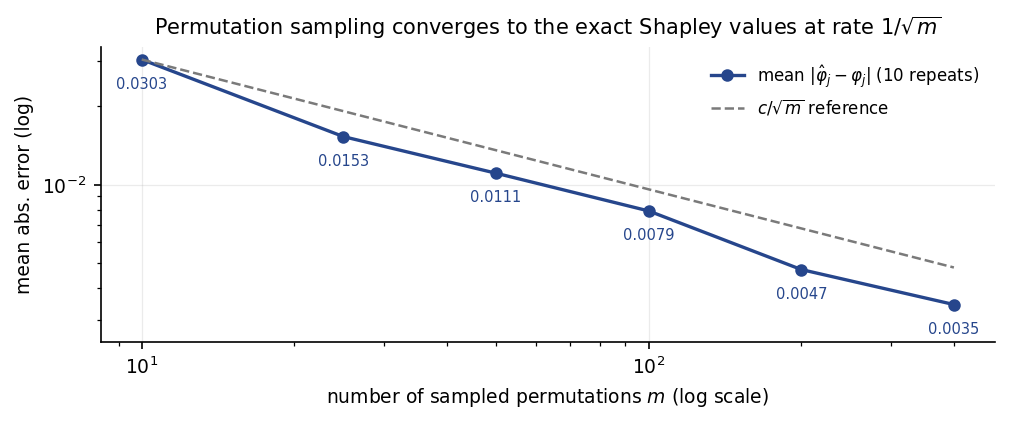
\includegraphics[width=0.9\textwidth,height=0.5\textheight,keepaspectratio]{a2_convergence.png}
  \end{center}
  \begin{takeaway}
    For the veteran instance, $m=25$ sampled orders already bring the mean absolute
    error to $0.015$ log-dollars ($\sim2\%$ of the largest $|\varphi_j|$); by $m=400$
    it is $0.0035$. The dashed $c/\sqrt{m}$ line confirms the rate: $\times4$ orders
    $\Rightarrow$ error halved ($0.0153 \to 0.0079$ from $m=25$ to $100$).
  \end{takeaway}
\end{frame}

\begin{frame}{Scaling up in practice: KernelSHAP, TreeSHAP, \texttt{shap}}
  \footnotesize
  \begin{block}{KernelSHAP in one idea (Lundberg \& Lee, 2017)}
    Efficiency suggests a regression: fit $v_x(S) \approx \sum_{j\in S}\varphi_j$
    by \textbf{weighted least squares} over sampled coalitions $S$, with the
    \emph{Shapley kernel} weight
    $\pi(S) = \frac{p-1}{\binom{p}{|S|}\,|S|\,(p-|S|)}$.
    With \emph{all} $2^p$ coalitions this WLS reproduces the exact Shapley values;
    with a sample it approximates them --- efficiently, because each sampled
    coalition informs all $p$ features at once.
  \end{block}
  \begin{readme}[TreeSHAP: exactness for free on tree ensembles]
    For trees, the expectations $E[f(x_S, X_{\bar S})]$ can be pushed \emph{through
    the tree structure}: exact Shapley values in polynomial time (roughly \#trees
    $\times$ \#leaves $\times$ depth$^2$ per instance) --- no $2^p$, no sampling
    noise. This is why boosted trees $+$ SHAP became the standard production pairing.
  \end{readme}
  \begin{takeaway}
    The \texttt{shap} package ships all of this (\texttt{TreeExplainer},
    \texttt{KernelExplainer}, the plots). We built everything from scratch so that
    \texttt{shap}'s output is a convenience, not a mystery --- it is not installed on
    the course machines, but one \texttt{pip install shap} away in Colab.
  \end{takeaway}
\end{frame}

\begin{frame}{Extended Exercise A2.1 --- Monte-Carlo Shapley from scratch [Python]}
\begin{longexercise}
  \scriptsize
  Implement permutation sampling for the veteran instance $x^\ast$ (row 188) and
  quantify its accuracy against the exact values from the previous slides.
  \begin{enumerate}
    \item Write \texttt{mc\_shapley(x, m, rng)}: sample $m$ orderings with
          \texttt{rng.permutation(p)}; for each, walk through the features,
          awarding each its change in $v$ (start the walk at $v(\varnothing)=0$).
    \item Run it with $m=100$ and \texttt{default\_rng(2024)}; tabulate
          $\hat\varphi_j$ against the exact $\varphi_j$ and report the mean and
          maximum absolute error.
    \item Estimate the error at $m\in\{25, 100, 400\}$ (average over $10$
          repeats). Does quadrupling $m$ halve the error?
    \item Compare total model calls of your $m=100$ run against exact
          enumeration at $p=6$. Which wins here, and when does that flip?
  \end{enumerate}
\end{longexercise}
\begin{labnote}[Run this live]
  \scriptsize
  The worked solution sits in \texttt{advanced\_02\_shapley\_lab.ipynb} under
  \emph{Lecture exercises --- worked Python solutions}: the cell headed
  \emph{Extended Exercise A2.1 --- Monte-Carlo Shapley from scratch [Python]}.
\end{labnote}
\end{frame}

\begin{frame}[fragile]{Solution --- Extended Exercise A2.1 (1/3)}
\begin{solutionbox}[Solution --- code: sampling arrival orders]
  \begin{lstlisting}[basicstyle=\ttfamily\scriptsize]
def mc_shapley(x, m, rng):                  # estimate all p values
    est = np.zeros(p)                       # running sum per player
    for _ in range(m):                      # m random arrival orders
        perm = rng.permutation(p)           # order, e.g. [3 0 5 1 4 2]
        S, v_prev = [], 0.0                 # empty room: v = 0
        for j in perm:                      # features arrive one by one
            v_new = v(tuple(S) + (int(j),), x)   # worth once j joins
            est[j] += v_new - v_prev        # credit j the jump in v
            v_prev = v_new                  # this order's new baseline
            S.append(int(j))                # j now counts as "known"
    return est / m                          # mean = unbiased phi-hat

rng = np.random.default_rng(2024)           # fresh seeded generator
est = mc_shapley(x_star, 100, rng)          # 100 orders = 600 v-calls
  \end{lstlisting}
  \textbf{Method.} One pass through an ordering costs $p$ evaluations of $v$ and
  awards every feature exactly once --- so each pass is one telescoping sample of
  \emph{all} $p$ Shapley values simultaneously.
\end{solutionbox}
\end{frame}

\begin{frame}{Solution --- Extended Exercise A2.1 (2/3)}
\begin{solutionbox}[Solution --- the $m{=}100$ run against the exact values]
  \begin{center}
  \begin{tabular}{@{}lrrrrrr@{}}
    \toprule
    & \texttt{Years} & \texttt{CHits} & \texttt{CRBI} & \texttt{Walks} & \texttt{Hits} & \texttt{PutOuts} \\
    \midrule
    $\hat\varphi_j$ ($m{=}100$) & $-0.5164$ & $+0.5408$ & $+0.5741$ & $-0.0496$ & $-0.1071$ & $+0.3145$ \\
    $\varphi_j$ (exact)         & $-0.5245$ & $+0.5626$ & $+0.5474$ & $-0.0452$ & $-0.1084$ & $+0.3244$ \\
    \bottomrule
  \end{tabular}
  \end{center}
  \textbf{Part 2 --- errors.} Mean absolute error $= 0.012$, maximum $= 0.027$
  (on \texttt{CRBI}) --- about $2$--$5\%$ of the leading attributions: every sign
  and the full ranking are already correct at $m=100$.

  \medskip
  \textbf{Part 3 --- rate.} Averaged over $10$ repeats: error $0.0153$ at $m=25$,
  $0.0079$ at $m=100$, $0.0035$ at $m=400$. Each quadrupling roughly halves the
  error --- the $1/\sqrt{m}$ signature of a Monte-Carlo mean.
\end{solutionbox}
\end{frame}

\begin{frame}{Solution --- Extended Exercise A2.1 (3/3)}
\begin{solutionbox}[Solution --- cost accounting and when sampling wins]
  \scriptsize
  \textbf{Part 4 --- model calls.}
  \begin{itemize}
    \item \textbf{Exact} at $p=6$: $2^p \cdot B = 64 \times 100 = 6\,400$ calls.
    \item \textbf{MC} at $m=100$: $m \cdot p \cdot B = 100 \times 6 \times 100
          = 60\,000$ calls --- \emph{nine times more}, for an approximate answer.
  \end{itemize}
  At $p=6$, exact enumeration wins outright. The flip is fast: exact doubles with
  every added feature ($2^{20}\cdot B \approx 10^{8}$ calls at $p=20$), while the
  MC budget $m\,p\,B$ grows only \emph{linearly} in $p$ --- at $p=20$ the same
  $m=100$ costs $200\,000$ calls, now $500\times$ cheaper than exact.

  \smallskip
  \textbf{Take-away.} Enumerate while you can ($p \lesssim 15$); sample when you
  must; and if the model is a tree ensemble, TreeSHAP gives exactness at neither
  price.
\end{solutionbox}
\begin{mistake}
  Judging convergence from a single run at one $m$: a lucky draw can look converged
  while another seed disagrees in the second decimal. Always repeat with several
  seeds (or track the standard error across orderings) before trusting
  $\hat\varphi_j$.
\end{mistake}
\end{frame}

% ============================================================
\section{Reading the Output}
% ============================================================

\begin{frame}{Local view: the waterfall of one prediction}
  \footnotesize
  \begin{center}
    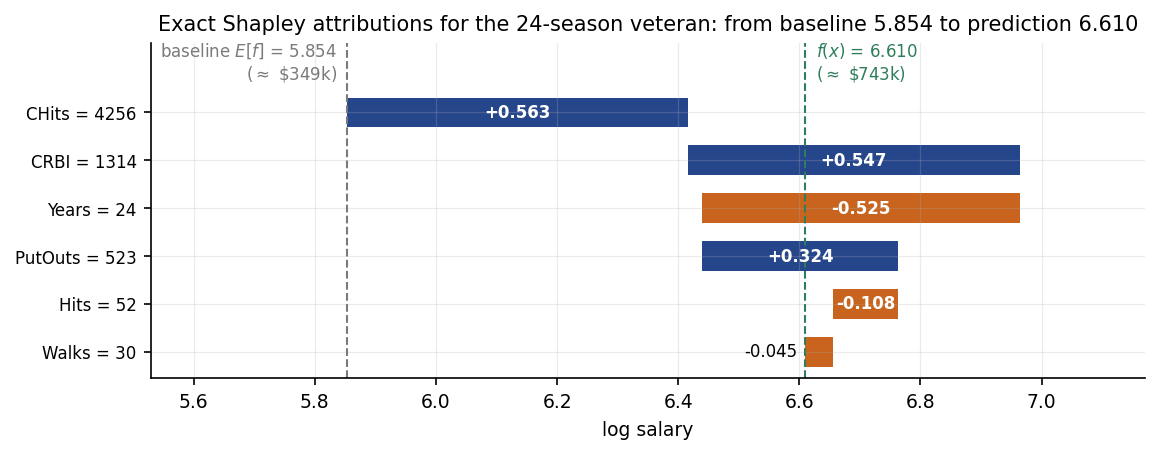
\includegraphics[width=0.9\textwidth,height=0.5\textheight,keepaspectratio]{a2_local_waterfall.png}
  \end{center}
  \begin{takeaway}
    Read it left to right: start at the baseline $5.854$ ($\approx\$349$k), add the six
    attributions in order of size, land exactly on $f(x)=6.610$ ($\approx\$743$k). The
    record career totals push up ($+0.563$, $+0.547$); being $24$ seasons old pushes
    down ($-0.525$); a weak current season ($52$ hits) subtracts another $-0.108$.
  \end{takeaway}
\end{frame}

\begin{frame}{Reading attributions on the log scale}
  \footnotesize
  Our model predicts \emph{log} salary, so attributions are additive in logs ---
  i.e.\ \textbf{multiplicative} in dollars.
  \begin{numexample}[The veteran's salary --- rebuilt factor by factor]
    \[
      \underbrace{349}_{\text{baseline}} \times
      \underbrace{e^{+0.563}}_{\texttt{CHits}:\ \times1.76} \times
      \underbrace{e^{+0.547}}_{\texttt{CRBI}:\ \times1.73} \times
      \underbrace{e^{-0.525}}_{\texttt{Years}:\ \times0.59} \times
      \underbrace{e^{+0.324}}_{\texttt{PutOuts}} \times
      \underbrace{e^{-0.108-0.045}}_{\texttt{Hits},\ \texttt{Walks}}
      \;\approx\; 743 \text{ (\$1\,000)}
    \]
    All six together: $e^{0.756} = 2.13$ --- this player is priced at
    \textbf{2.1 times} the baseline salary, and the waterfall says exactly why.
  \end{numexample}
  \begin{readme}[Units checklist before you present]
    (i) \emph{Which output?} log salary, probability, log-odds, \texteuro?
    (ii) \emph{Which baseline?} $\varphi_0=5.854$ is the mean prediction over the
    $B=100$ background rows --- a different background moves every $\varphi_j$.
    (iii) \emph{Sanity sum:} $\varphi_0 + \sum_j\varphi_j$ must equal $f(x)$.
  \end{readme}
  \begin{labnote}
    Notebook \S5 rebuilds this waterfall and lets you swap instance and background ---
    watch the baseline and every bar move together.
  \end{labnote}
\end{frame}

\begin{frame}{Global view: mean $|\varphi_j|$ vs.\ permutation importance}
  \footnotesize
  \begin{center}
    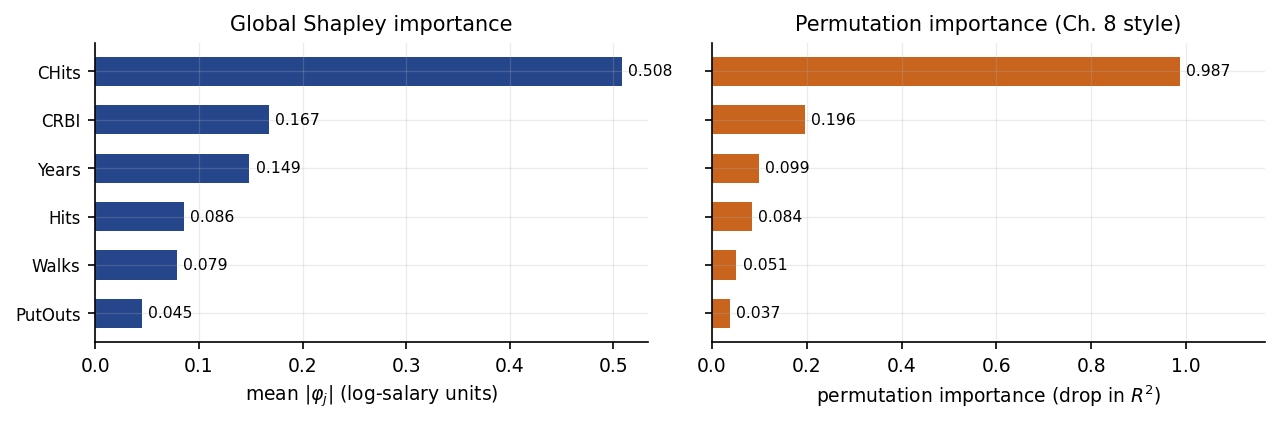
\includegraphics[width=0.94\textwidth,height=0.46\textheight,keepaspectratio]{a2_global_importance.png}
  \end{center}
  \begin{takeaway}
    Both rankings agree here: \texttt{CHits} dominates, then \texttt{CRBI} and
    \texttt{Years}. But the \emph{numbers} answer different questions: mean
    $|\varphi_j|$ ($0.508$ for \texttt{CHits}) is an average \textbf{contribution in
    log-salary units}; permutation importance ($0.987$) is the \textbf{drop in $R^2$}
    when the feature is scrambled (Ch.\ 8). Under correlation they can diverge:
    permuting \texttt{CHits} also destroys information shared with \texttt{CRBI}
    ($r=0.947$), inflating its apparent solo importance.
  \end{takeaway}
\end{frame}

\begin{frame}{Dependence view: how an attribution varies with its feature}
  \footnotesize
  \begin{center}
    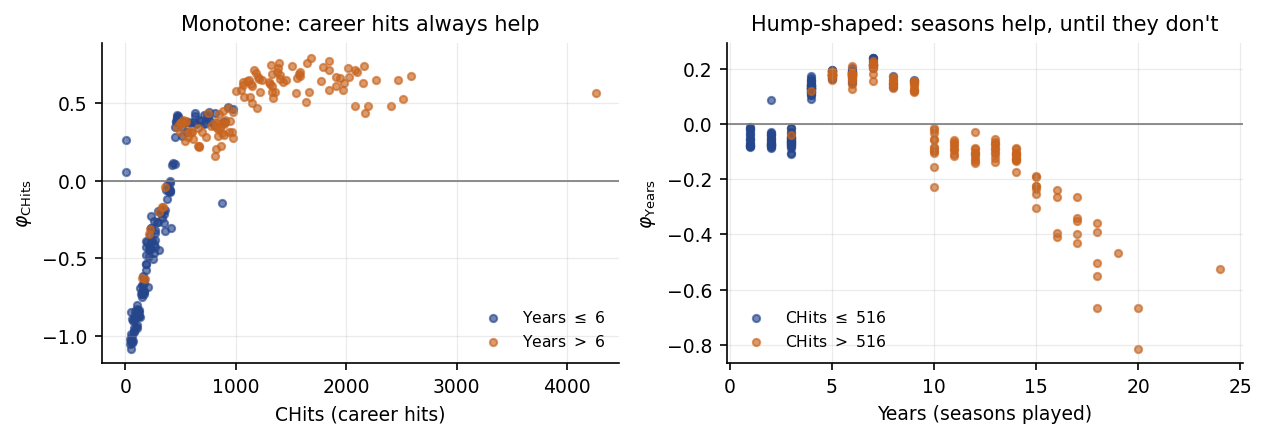
\includegraphics[width=0.94\textwidth,height=0.46\textheight,keepaspectratio]{a2_dependence.png}
  \end{center}
  \begin{takeaway}
    Left: $\varphi_{\texttt{CHits}}$ rises monotonically --- mean $-0.70$ below $250$
    career hits, $+0.63$ above $1\,000$: career volume always pays. Right:
    $\varphi_{\texttt{Years}}$ is \textbf{hump-shaped} --- $+0.19$ around seasons
    $5$--$7$, falling to $-0.45$ beyond $15$: \emph{given} career totals, extra seasons
    mean less production per season. Vertical spread at a fixed $x$-value (and the
    colour split) is the fingerprint of \textbf{interactions}.
  \end{takeaway}
\end{frame}

\begin{frame}{Exercise A2.5 --- Explain another player [Python]}
\begin{exercise}
  Row $0$ of the cleaned data is a $14$-season veteran: \texttt{Years} $=14$,
  \texttt{CHits} $=835$, \texttt{CRBI} $=414$, \texttt{Walks} $=39$,
  \texttt{Hits} $=81$, \texttt{PutOuts} $=632$; actual salary $\$475$k.
  With the fitted model and \texttt{exact\_shapley} from the lab:
  \begin{enumerate}
    \item Compute $f(x)$ and the six exact attributions $\varphi_j$.
    \item Verify efficiency: $\sum_j\varphi_j = f(x)-\varphi_0$.
    \item Name the largest positive and the largest negative contribution and
          restate each as a multiplicative salary factor $e^{\varphi_j}$.
  \end{enumerate}
\end{exercise}
\begin{labnote}[Run this live]
  The worked solution sits in \texttt{advanced\_02\_shapley\_lab.ipynb} under
  \emph{Lecture exercises --- worked Python solutions}: the cell headed
  \emph{Exercise A2.5 --- Explain another player [Python]}.
\end{labnote}
\end{frame}

\begin{frame}{Solution --- Exercise A2.5}
\begin{solutionbox}
  \scriptsize
  \textbf{Part 1 --- the numbers.} $f(x) = 6.167$ log-dollars $\approx \$477$k
  (actual: $\$475$k --- the model is nearly on the money here).
  \begin{center}
  \begin{tabular}{@{}lrrrrrr@{}}
    \toprule
    & \texttt{CHits} & \texttt{PutOuts} & \texttt{CRBI} & \texttt{Walks} & \texttt{Hits} & \texttt{Years} \\
    \midrule
    $\varphi_j$ & $+0.287$ & $+0.176$ & $+0.112$ & $-0.037$ & $-0.100$ & $-0.125$ \\
    \bottomrule
  \end{tabular}
  \end{center}
  \textbf{Part 2 --- efficiency.} $\sum_j\varphi_j = 0.313$ and
  $f(x)-\varphi_0 = 6.167-5.854 = 0.313$: equal to machine precision. $\checkmark$

  \smallskip
  \textbf{Part 3 --- reading.} Largest positive: \texttt{CHits} $=+0.287$, a factor
  $e^{0.287}\approx 1.33$ --- a solid career record raises the predicted salary by a
  third. Largest negative: \texttt{Years} $=-0.125$, factor $e^{-0.125}\approx0.88$
  --- the same late-career discount we saw in the dependence plot ($14$ seasons sits
  on its downslope), only milder than the record-holder's $-0.525$ at $24$ seasons.
\end{solutionbox}
\begin{mistake}
  Comparing $\varphi_j$ across explanations computed with \emph{different
  backgrounds}: attributions are shares of $f(x)-\varphi_0$, so changing $\varphi_0$
  rescales the whole decomposition. One report, one background.
\end{mistake}
\end{frame}

% ============================================================
\section{Pitfalls}
% ============================================================

\begin{frame}{Pitfall 1: correlated features put the model off-manifold}
  \scriptsize
  \begin{center}
    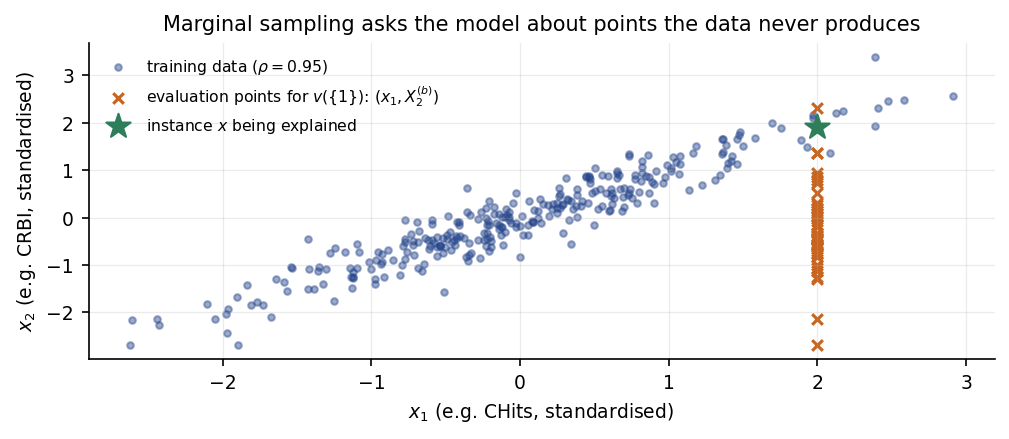
\includegraphics[width=0.8\textwidth,height=0.32\textheight,keepaspectratio]{a2_offmanifold.png}
  \end{center}
  \vspace{-2pt}
  \begin{takeaway}
    Marginal sampling pins $x_1$ and draws $x_2$ from the background --- the orange
    crosses. With $\rho=0.95$ most sit \textbf{outside} the data ridge: we query the
    model where it never saw data (in \texttt{Hitters},
    $r_{\texttt{CHits},\texttt{CRBI}}=0.947$, so $v(S)$ averages over impossible
    careers like $4\,256$ hits with $3$ RBI). The attributions inherit whatever the
    model \emph{extrapolates} out there.
  \end{takeaway}
  \begin{mistake}
    Trusting fine differences between correlated features' attributions: that split
    rests exactly on the off-manifold region. Robust practice: report the
    \textbf{group attribution} $\varphi_{\texttt{CHits}}+\varphi_{\texttt{CRBI}}$, or
    switch to a conditional value function and accept its price (Exercise A2.4).
  \end{mistake}
\end{frame}

\begin{frame}{Pitfall 2: an explanation is not a cause}
  \footnotesize
  $\varphi_{\texttt{Years}} = -0.525$ for the veteran. Three readings --- only one
  is licensed:
  \begin{readme}[What the number does and does not say]
    \begin{itemize}
      \item \checkmark\ \textbf{Model-mechanical:} pinning \texttt{Years} $=24$
            (vs.\ background values) lowers the model's average output by $0.525$ ---
            a statement about $f$ and the background, nothing else.
      \item $\times$ \textbf{Worldly-causal:} ``playing fewer seasons would have
            raised his salary'' --- Shapley intervenes on the \emph{model's inputs},
            not on the world; no design (randomisation, instruments) supports this.
      \item $\times$ \textbf{Recourse:} ``to be paid more, reduce \texttt{Years}''
            --- feature values cannot be moved independently in reality
            (\texttt{Years} drags \texttt{CHits}, $r=0.898$), and the model would be
            refitted on any new regime anyway.
    \end{itemize}
  \end{readme}
  \begin{takeaway}
    Shapley explanations answer ``\textbf{how did the model use its inputs}'', never
    ``what should the customer change''. Recourse and causal claims need causal
    tools --- a different module, different assumptions.
  \end{takeaway}
\end{frame}

\begin{frame}{Pitfall 3: attributions move when the model is retrained}
  \footnotesize
  \begin{numexample}[Same data and accuracy --- different explanations]
    Two stochastic refits (\texttt{subsample=0.7}, seeds $1$ and $2$) both reach
    train $R^2 \approx 0.96$. Exact Shapley for the veteran:
    \begin{center}
    \begin{tabular}{@{}lccc@{}}
      \toprule
      & $\varphi_{\texttt{CHits}}$ & $\varphi_{\texttt{CRBI}}$ & sum of the pair \\
      \midrule
      refit, seed 1 & $+0.702$ & $+0.521$ & $+1.223$ \\
      refit, seed 2 & $+0.600$ & $+0.545$ & $+1.146$ \\
      \bottomrule
    \end{tabular}
    \end{center}
    $\varphi_{\texttt{CHits}}$ swings by $0.10$ ($\sim15\%$) between two equally
    accurate models; the \textbf{pair's sum} moves far less. Correlated features are
    interchangeable to the fit --- so the fit chooses arbitrarily, and the
    attribution follows.
  \end{numexample}
  \begin{takeaway}[Version everything the explanation depends on]
    Model artefact, background sample, seed and library version are all inputs to
    $\varphi_j$, so all four belong in the documentation. A declined customer who
    reapplies must not receive contradictory ``principal reasons'' because a nightly
    retrain shuffled credit between two collinear features.
  \end{takeaway}
\end{frame}

\begin{frame}{Extended Exercise A2.2 --- Designing a credit-explanation pipeline [Integrative]}
\begin{longexercise}
  A bank declines consumer loans with a gradient-boosted classifier
  ($p=40$ features; \texttt{income}, \texttt{debt\_to\_income},
  \texttt{n\_open\_lines}, \texttt{history\_length} form a correlated cluster).
  Regulation requires the top-3 ``principal reasons'' on every decline notice.
  Design the pipeline:
  \begin{enumerate}
    \item Local or global explanations for the notice --- and what do you keep the
          global ones for?
    \item Choose and defend a \textbf{background}: all applicants, approved
          applicants, or a single ``average customer'' row.
    \item Exact, permutation-sampling, KernelSHAP or TreeSHAP --- pick one and
          justify with the cost arithmetic of this module.
    \item The correlated cluster: one concrete danger for the reason codes, and
          one mitigation.
    \item The applicant replies: ``so if I raise my income by \texteuro5\,000 I
          will be approved?'' --- draft the honest two-sentence answer.
  \end{enumerate}
\end{longexercise}
\end{frame}

\begin{frame}{Solution --- Extended Exercise A2.2 (1/2)}
\begin{solutionbox}[Solution --- parts 1--3: the architecture]
  \textbf{Part 1 --- local for the notice, global for governance.} The notice
  explains \emph{one} decision $\Rightarrow$ local $\varphi_j$ for that applicant;
  the top-3 negative attributions map to standardised reason codes. Global mean
  $|\varphi_j|$ goes to validation: driver stability over time, drift alarms,
  fair-lending review.

  \smallskip
  \textbf{Part 2 --- background = approved applicants.} The legal question is
  ``why were \emph{you} declined \emph{rather than approved}'', so the reference
  population should be the approved pool: $\varphi_0$ becomes the average score of
  approved customers and negative $\varphi_j$'s read ``what separates you from
  them''. (All-applicants blurs the question; a single average row is not a
  distribution at all and makes the explanation hostage to one synthetic point.)

  \smallskip
  \textbf{Part 3 --- TreeSHAP.} $p=40$ kills exact enumeration
  ($2^{40}\approx10^{12}$ coalitions); permutation sampling and KernelSHAP cost
  $m\,p\,B$ model calls \emph{per applicant} with sampling noise on top --- awkward
  when notices must be reproducible. The model is a tree ensemble, so TreeSHAP is
  exact, fast and deterministic: the only defensible choice here.
\end{solutionbox}
\end{frame}

\begin{frame}{Solution --- Extended Exercise A2.2 (2/2)}
\begin{solutionbox}[Solution --- parts 4--5: correlation and the customer's question]
  \textbf{Part 4 --- the cluster danger.} Credit for the debt burden can split
  arbitrarily across \texttt{income}, \texttt{debt\_to\_income},
  \texttt{n\_open\_lines}: after a routine retrain the top-3 list can swap
  ``income too low'' for ``too many open lines'' with \emph{no change in the
  applicant} --- inconsistent notices, regulatory exposure. \textbf{Mitigation:}
  define reason codes on \textbf{feature groups} (sum the cluster's $\varphi_j$'s
  --- efficiency makes group sums well-defined), and freeze model + background +
  seed per reporting period.

  \smallskip
  \textbf{Part 5 --- the honest answer.} ``The reasons describe how our current
  model weighed your data compared with approved customers; they are not a promise
  that changing one number changes the decision. A higher income would enter a new
  application, but the outcome depends on your whole profile at that time.''
\end{solutionbox}
\begin{mistake}
  Publishing reason codes from raw per-feature attributions in a correlated feature
  space. The maths is exact, but the \emph{split within a cluster} is a modelling
  artefact --- group first, then explain.
\end{mistake}
\end{frame}

% ============================================================
\section{Summary}
% ============================================================

\begin{frame}{Module A2 in one slide}
  \begin{block}{What we accomplished}
    Exact, axiom-backed feature attributions for a black-box model --- built
    entirely from scratch.
  \end{block}
  \begin{itemize}
    \item Local vs.\ global explanations, and what an attribution must promise.
    \item Cooperative games: value functions, marginal contributions, a fully
          worked three-player division ($170/110/20$).
    \item The Shapley value: the $\frac{|S|!(p-|S|-1)!}{p!}$ formula, four axioms,
          uniqueness.
    \item Models as games: $v_x(S)$ via background samples; marginal vs.\
          conditional.
    \item Computation: exact $2^p$ enumeration ($p=6$: $64$ coalitions),
          $1/\sqrt{m}$ Monte-Carlo, KernelSHAP, TreeSHAP.
    \item Reading output: waterfall ($349\text{k}\to743\text{k}$), mean
          $|\varphi_j|$ vs.\ permutation importance, dependence plots.
    \item Pitfalls: off-manifold sampling, explanation $\neq$ causation,
          retrain instability.
  \end{itemize}
\end{frame}

\begin{frame}{Key formulas at a glance}
  \footnotesize
  \begin{description}
    \item[Shapley value] $\varphi_j=\displaystyle\sum_{S\subseteq\mathcal{P}\setminus\{j\}}
      \frac{|S|!\,(p-|S|-1)!}{p!}\bigl(v(S\cup\{j\})-v(S)\bigr)$.
    \item[Weight identity] $\dfrac{|S|!\,(p-|S|-1)!}{p!} = \dfrac1p\binom{p-1}{|S|}^{-1}
      = \Pr(\text{$j$ arrives right after }S)$; weights sum to $1$.
    \item[Order form] $\varphi_j = E_\pi\bigl[v(\mathrm{pre}_\pi(j)\cup\{j\})
      - v(\mathrm{pre}_\pi(j))\bigr]$ --- basis of Monte-Carlo sampling, error
      $\propto 1/\sqrt{m}$.
    \item[Model as game] $v_x(S) = E\bigl[f(x_S, X_{\bar S})\bigr] - \varphi_0$
      (marginal) \;vs.\; $E\bigl[f(X)\mid X_S=x_S\bigr] - \varphi_0$ (conditional).
    \item[Local accuracy] $f(x) = \varphi_0 + \sum_{j=1}^p \varphi_j$ \ (efficiency,
      applied to the prediction game).
    \item[Global importance] $I_j = \frac1n\sum_{i=1}^n |\varphi_j^{(i)}|$ \ (mean
      absolute attribution).
    \item[KernelSHAP kernel] $\pi(S) = \dfrac{p-1}{\binom{p}{|S|}\,|S|\,(p-|S|)}$ \
      (WLS over coalitions recovers $\varphi$).
  \end{description}
\end{frame}

\begin{frame}{Vocabulary checklist}
  \footnotesize
  \begin{tabular}{ll}
    \toprule
    \textbf{Term} & \textbf{Meaning} \\
    \midrule
    Coalition $S$ & subset of players / features treated as ``present'' \\
    Value function $v(S)$ & worth of a coalition; for models: expected prediction given $x_S$ \\
    Marginal contribution & $v(S\cup\{j\})-v(S)$: what $j$ adds on arrival \\
    Shapley value $\varphi_j$ & weighted average of $j$'s marginal contributions \\
    Efficiency / local accuracy & attributions sum exactly to $f(x)-\varphi_0$ \\
    Dummy axiom & unused player gets $0$ \\
    Baseline $\varphi_0$ & average prediction over the background sample \\
    Background sample & data rows standing in for ``unknown'' features \\
    Marginal vs.\ conditional & break vs.\ respect feature correlations in $v(S)$ \\
    Permutation sampling & Monte-Carlo Shapley from random arrival orders \\
    KernelSHAP / TreeSHAP & WLS approximation / exact polynomial-time trees \\
    Waterfall plot & one prediction rebuilt attribution by attribution \\
    Mean $|\varphi_j|$ & global importance from local attributions \\
    Off-manifold evaluation & querying the model at impossible feature combinations \\
    \bottomrule
  \end{tabular}
\end{frame}

\begin{frame}{Decision rules of thumb}
  \begin{itemize}
    \item $p \lesssim 15$ and a cheap model $\Rightarrow$ \textbf{enumerate exactly};
          verify efficiency to machine precision as a pipeline test.
    \item Tree ensemble $\Rightarrow$ \textbf{TreeSHAP} (exact, deterministic);
          anything else at large $p$ $\Rightarrow$ KernelSHAP or permutation
          sampling with repeats and reported Monte-Carlo error.
    \item Choose the \textbf{background to match the question} (``compared to
          whom?'') --- and keep it fixed across every explanation you compare.
    \item Correlated feature clusters $\Rightarrow$ report \textbf{group sums} of
          attributions; distrust the within-cluster split.
    \item Always state the \textbf{output scale} (log, probability, log-odds) and
          the baseline next to any $\varphi_j$.
    \item Say ``the \emph{model} used $x_j$ this way'' --- never ``$x_j$
          \emph{caused} the outcome'' and never ``change $x_j$ to change the
          decision''.
  \end{itemize}
\end{frame}

\begin{frame}{Common pitfalls}
  \begin{alertblock}{Don't}
    \begin{enumerate}
      \item Read Shapley values causally or hand them to customers as recourse
            advice.
      \item Compare attributions computed against different backgrounds, model
            versions or seeds.
      \item Trust the credit split \emph{within} a correlated cluster
            (off-manifold arithmetic decides it).
      \item Report sampled Shapley values without a Monte-Carlo error estimate.
      \item Confuse mean $|\varphi_j|$ with permutation importance --- different
            units, different question.
      \item Treat the explanation as a property of reality --- it is a property of
            \emph{one fitted model} plus \emph{one value-function choice}.
    \end{enumerate}
  \end{alertblock}
\end{frame}

\begin{frame}{Self-check questions}
  \footnotesize
  \begin{readme}[Can you answer these without the slides?]
    \begin{enumerate}
      \item Why is the Shapley weight $|S|!\,(p-|S|-1)!/p!$ exactly the probability
            that $j$ arrives right after the coalition $S$?
      \item State the four axioms; which one turns Shapley values into an exact
            decomposition of $f(x)-\varphi_0$?
      \item In the consultancy game, why does C earn $20$ despite
            $v(\{C\})=0$?
      \item What breaks if you estimate $v_x(S)$ with marginal sampling when
            $r_{\texttt{CHits},\texttt{CRBI}}=0.947$?
      \item You quadruple the number of sampled orderings. What happens to the
            estimation error, and why?
      \item Why did $\varphi_{\texttt{CHits}}$ change from $0.702$ to $0.600$
            across two retrains --- and what stayed (almost) put?
    \end{enumerate}
  \end{readme}
  \begin{takeaway}
    If question 4 or 6 feels shaky, re-read the Pitfalls section --- that is where
    explanation projects fail in practice.
  \end{takeaway}
\end{frame}

% ============================================================
\appendix
\AtBeginSection[]{}
\section{Appendix: optional and advanced material}
% ============================================================

\begin{frame}{Appendix --- what is in here, and why}
  \small
  Nothing in the appendix is needed to follow the module: each slide is a
  formal derivation, a longer worked exercise, or a side topic. Read it when
  you want the full story, or when a later project sends you back here.
  \begin{block}{Contents of the appendix}
    \begin{itemize}
      \item \textbf{The weights, derived} --- the counting argument behind
            $|S|!(p-|S|-1)!/p!$; moved out because the main deck only needs the
            \emph{reading} of the weight, not its proof.
      \item \textbf{Efficiency, proved} --- the telescoping argument; two lines,
            but a proof nonetheless.
      \item \textbf{KernelSHAP as weighted regression} --- the algebra sketch
            behind the one-slide summary in the main deck.
      \item \textbf{Estimating conditional value functions} --- why the
            ``respect-the-data'' option is genuinely hard; for readers heading
            into research or high-stakes deployment.
      \item \textbf{Drill exercise (glove game)} --- one more full Shapley
            computation for exam practice, with solution.
    \end{itemize}
  \end{block}
\end{frame}

\begin{frame}{The weights, derived from random arrival orders}
  \footnotesize
  \begin{block}{Claim}
    Under a uniformly random ordering $\pi$ of $\mathcal{P}$,
    \[
      \Pr\bigl(\mathrm{pre}_\pi(j) = S\bigr) \;=\; \frac{|S|!\,(p-|S|-1)!}{p!}
      \qquad\text{for any } S \subseteq \mathcal{P}\setminus\{j\}.
    \]
  \end{block}
  \begin{readme}[The counting]
    An ordering with $\mathrm{pre}_\pi(j)=S$ is built by: arranging the $|S|$
    members of $S$ before $j$ ($|S|!$ ways), then $j$ (fixed), then the remaining
    $p-|S|-1$ players ($\,(p-|S|-1)!$ ways). Total favourable orderings:
    $|S|!\,(p-|S|-1)!$ out of $p!$ equally likely ones. $\blacksquare$
  \end{readme}
  \begin{takeaway}
    Hence
    $\varphi_j=\sum_S \Pr(\mathrm{pre}_\pi(j)=S)\,\bigl(v(S\cup\{j\})-v(S)\bigr)
    = E_\pi\bigl[\text{$j$'s arrival contribution}\bigr]$: the subset formula and
    the order-average are the \emph{same object}, which is why permutation sampling
    is unbiased.
  \end{takeaway}
\end{frame}

\begin{frame}{Efficiency, proved in two lines}
  \footnotesize
  \begin{block}{Claim}
    $\sum_{j=1}^{p}\varphi_j = v(\mathcal{P}) - v(\varnothing)$.
  \end{block}
  \begin{readme}[Telescoping]
    Fix any ordering $\pi = (j_1,\dots,j_p)$ and sum the arrival contributions
    \emph{along this one ordering}:
    \[
      \sum_{k=1}^{p}\bigl[v(\{j_1,\dots,j_k\}) - v(\{j_1,\dots,j_{k-1}\})\bigr]
      = v(\mathcal{P}) - v(\varnothing),
    \]
    because every intermediate $v(\cdot)$ appears once with $+$ and once with $-$.
    The sum is the same for \emph{every} ordering, and averaging over $\pi$ (which is
    what $\sum_j\varphi_j$ does, by the previous slide) preserves it. $\blacksquare$
  \end{readme}
  \begin{takeaway}
    Symmetry and dummy are equally quick from the order view; only
    \emph{uniqueness} needs real work --- see Shapley (1953).
  \end{takeaway}
\end{frame}

\begin{frame}{KernelSHAP as a weighted regression (sketch)}
  \footnotesize
  Represent a coalition $S$ by $z\in\{0,1\}^p$ and posit the \textbf{additive
  surrogate} $g(z)=\varphi_0+\sum_j \varphi_j z_j$.
  \begin{block}{The estimator}
    \[
      \hat\varphi = \arg\min_{\varphi}\ \sum_{z}\ \pi(z)\,
      \bigl(v_x(z) - g(z)\bigr)^2,
      \qquad
      \pi(z)=\frac{p-1}{\binom{p}{|z|}\,|z|\,(p-|z|)},
    \]
    with $g(\mathbf{0})=0$ and $g(\mathbf{1})=f(x)-\varphi_0$ imposed exactly
    (the kernel is $+\infty$ there, so they act as constraints).
  \end{block}
  \begin{readme}
    \begin{itemize}
      \item Lundberg \& Lee (2017) show: with \emph{all} $2^p$ coalitions, the WLS
            solution equals the Shapley values --- the kernel is reverse-engineered
            so that this holds.
      \item In practice one samples coalitions $\propto\pi(z)$; each sampled $v_x(z)$
            informs \emph{all} $p$ coefficients simultaneously --- the efficiency
            advantage over order sampling.
      \item Caveat: sampled KernelSHAP is still Monte-Carlo --- report its error, as
            with permutation sampling.
    \end{itemize}
  \end{readme}
\end{frame}

\begin{frame}{Estimating conditional value functions is genuinely hard}
  \footnotesize
  The conditional choice $v_x(S)=E[f(X)\mid X_S=x_S]-\varphi_0$ needs the
  conditional law of $X_{\bar S}$ given $X_S = x_S$ --- for \emph{every} $S$.
  \begin{readme}[The estimation menu (Aas et al.\ 2021)]
    \begin{itemize}
      \item \textbf{Empirical / kernel:} reweight background rows by closeness to
            $x_S$ --- struggles beyond a few dimensions.
      \item \textbf{Parametric:} assume Gaussian (or copula) features, condition in
            closed form --- clean, but a real assumption about the data.
      \item \textbf{Generative / surrogate:} train a model of $X_{\bar S}\mid X_S$
            --- now the \emph{explanation} has its own model risk.
      \item \textbf{Path-dependent TreeSHAP:} approximates conditioning with the
            tree's split cover statistics --- fast, but neither cleanly marginal nor
            cleanly conditional.
    \end{itemize}
  \end{readme}
  \begin{takeaway}
    This is why the marginal form is the pragmatic default: its estimator is a plain
    average. The price is Pitfall 1 --- choose which price you pay, and \textbf{say
    so in the report}.
  \end{takeaway}
\end{frame}

\begin{frame}{Exercise A2.6 --- The glove game (drill) [Math]}
\begin{exercise}
  Players $1$ and $2$ each own a \textbf{left} glove; player $3$ owns a
  \textbf{right} glove. A coalition earns $1$ if it holds at least one complete
  pair (a left \emph{and} a right glove), else $0$:
  $v(S)=1$ iff $3\in S$ and $S\cap\{1,2\}\neq\varnothing$.
  \begin{enumerate}
    \item Write out $v(S)$ for all eight coalitions.
    \item Compute $\varphi_3$ with the subset formula ($p=3$ weights
          $\tfrac13,\tfrac16,\tfrac16,\tfrac13$).
    \item Deduce $\varphi_1$ and $\varphi_2$ \emph{without} further computation,
          naming the axioms you use.
  \end{enumerate}
\end{exercise}
\end{frame}

\begin{frame}{Solution --- Exercise A2.6}
\begin{solutionbox}
  \textbf{Part 1.} $v=0$ for $\varnothing,\{1\},\{2\},\{3\},\{1,2\}$; \
  $v=1$ for $\{1,3\},\{2,3\},\{1,2,3\}$.

  \smallskip
  \textbf{Part 2 --- $\varphi_3$ via the four coalitions $S\subseteq\{1,2\}$:}
  \[
    \varphi_3 = \tfrac13\underbrace{(0-0)}_{S=\varnothing}
              + \tfrac16\underbrace{(1-0)}_{S=\{1\}}
              + \tfrac16\underbrace{(1-0)}_{S=\{2\}}
              + \tfrac13\underbrace{(1-0)}_{S=\{1,2\}}
    = \tfrac16+\tfrac16+\tfrac13 = \tfrac{2}{3}.
  \]
  \textbf{Part 3.} Players $1$ and $2$ are interchangeable in $v$
  ($v(S\cup\{1\})=v(S\cup\{2\})$ for every $S$ avoiding both), so
  \textbf{symmetry} gives $\varphi_1=\varphi_2$; \textbf{efficiency} gives
  $\varphi_1+\varphi_2+\varphi_3 = v(\mathcal{P})=1$, hence
  $\varphi_1=\varphi_2=\tfrac{1}{2}\bigl(1-\tfrac23\bigr)=\tfrac16$.

  \smallskip
  \textbf{Take-away.} Scarcity is worth money: the single right glove earns
  $\tfrac23$, four times each plentiful left glove --- the value prices
  \emph{replaceability}, exactly what it will later do with correlated features.
\end{solutionbox}
\begin{mistake}
  Splitting $1$ as $\tfrac13$ each ``because there are three players'': equal split
  ignores that removing player $1$ barely matters ($\{2,3\}$ still earns $1$) while
  removing player $3$ zeroes the game.
\end{mistake}
\end{frame}

\end{document}
